\documentclass[9pt]{beamer}
\usepackage[T1]{fontenc}
\usepackage[english]{babel}
\usepackage{xcolor}
\usepackage{amsfonts}
\usepackage{amsmath}
\usepackage{amssymb}
\usepackage{mathtools}
\usepackage{blkarray}
\usepackage{bm}
\usepackage{physics}
\usepackage{etoolbox}
\usepackage{eqparbox}
\usepackage{graphicx}

% Fonts
\renewcommand{\rmdefault}{ptm}
\renewcommand{\sfdefault}{phv}

% Spacing
\setlength\parindent{0pt}
\setlength\parskip{1ex plus 1ex minus 0.5ex}

% Basic notation
\DeclareMathOperator*{\argmax}{arg\,max}
\DeclareMathOperator*{\argmin}{arg\,min}
\renewcommand\d{\mathop{}\!\textnormal{\slshape d}}
\newcommand\eye{\mathop{}\!\mathbb{I}}
\newcommand\defined{\doteq}
\newcommand\upto{\stackrel{+}{=}}
\newcommand\without{\setminus}
\newcommand{\describe}[3][0pt]{\hspace*{.12em}\underbracket[0.5pt][1pt]{#2\hspace*{#1}}_\text{#3}}
\newcommand{\describel}[2]{\Shortunderstack[l]{$\underbracket[1pt][0pt]{#1}$ \raisebox{.8ex}{\scriptsize\rlap{#2}}}}
\newcommand{\changes}[1]{\underbracket[1pt][0pt]{#1}}

% Equation
\makeatletter
\newcommand{\removeParBefore}{\ifvmode\vspace*{-\baselineskip}\setlength{\parskip}{0ex}\fi}
\newcommand{\removeParAfter}{\@ifnextchar\par\@gobble\relax}
\newcommand{\eq}{\begingroup\removeParBefore\endlinechar=32 \eqinner}
\newcommand{\eqinner}[2][aligned]{\endlinechar=32%
\begin{gather}\begin{#1}#2\end{#1}\end{gather}\endgroup\removeParAfter}
\makeatother

% Density
\DeclareDocumentCommand{\p}{ D<>{p} D<>{} r() }{
\def\content{#3}\patchcmd{\content}{|}{\;#2\vert\;}{}{}
\ensuremath{#1 #2(\content #2)}}

% Probability
\DeclareDocumentCommand{\P}{ D<>{P} D<>{\big} r() }{
\def\content{#3}\patchcmd{\content}{|}{\;#2\vert\;}{}{}
\ensuremath{\operatorname{#1}#2(\content #2)}}

% Expectation
\DeclareDocumentCommand{\E}{ D<>{E} E{_}{{}} D<>{\big} r[] }{
\def\content{#4}\patchcmd{\content}{|}{\;#3\vert\;}{}{}
\ensuremath{\operatorname{#1}_{#2}#3[\content #3]}}

% Divergence
\DeclareDocumentCommand{\D}{ D<>{D} D<>{\big} r[] }{
\def\content{#3}\patchcmd{\content}{||}{\;#2\|\;}{}{}
\ensuremath{\operatorname{#1}\!#2[\content #2]}}

% Distributions
\NewDocumentCommand{\Nor}{ r() }{\P<Normal>](#1)}
\NewDocumentCommand{\Cat}{ r() }{\P<Cat>](#1)}
\NewDocumentCommand{\Bin}{ r() }{\P<Bin>](#1)}
\NewDocumentCommand{\Bet}{ r() }{\P<Beta>](#1)}
\NewDocumentCommand{\Ber}{ r() }{\P<Bernoulli>(#1)}
\NewDocumentCommand{\Dir}{ r() }{\P<Dir>(#1)}

% Information
\DeclareDocumentCommand{\KL}{ D<>{\big} r[] }{\D<KL><#1>[#2]}
\DeclareDocumentCommand{\H}{ D<>{\big} r[] }{\E<H><#1>[#2]}
\DeclareDocumentCommand{\I}{ D<>{\big} r[] }{\E<I><#1>[#2]}

% Symbols
\newcommand{\cmark}{\textcolor{green}{\ding{51}}}
\newcommand{\xmark}{\textcolor{red}{\ding{55}}}

% Shortcuts
\DeclareDocumentCommand{\lnpp}{ D<>{} r() }{
\ensuremath{\p<\ln p_\phi><#1>(#2)}}
\DeclareDocumentCommand{\pp}{ D<>{} r() }{
\ensuremath{\p<p_\phi><#1>(#2)}}
\DeclareDocumentCommand{\qp}{ D<>{} r() }{
\ensuremath{\p<q_\phi><#1>(#2)}}
\DeclareDocumentCommand{\SymLogNormal}{ D<>{} r() }{
\ensuremath{\p<\operatorname{SymLogNormal}><#1>(#2)}}
\newcommand{\sign}{\operatorname{sign}}
% \newcommand{\abs}{\operatorname{abs}}
\newcommand{\eps}{\epsilon}
% \newcommand{\erf}{\operatorname{erf}}
\newcommand{\fot}{\textstyle\frac{1}{2}}
\newcommand{\symlog}{\ensuremath{\operatorname{symlog}}}
\newcommand{\symexp}{\ensuremath{\operatorname{symexp}}}
\newcommand{\twohot}{\ensuremath{\operatorname{twohot}}}
\newcommand{\sg}{\ensuremath{\operatorname{sg}}}
\newcommand{\softmax}{\operatorname{softmax}}
\newcommand{\logsoftmax}{\operatorname{log\,softmax}}
\newcommand{\EMA}{\operatorname{EMA}}
\newcommand{\Per}{\operatorname{Per}}
\newcommand{\ema}{\operatorname{ema}}
\newcommand{\per}{\operatorname{per}}

\usepackage{tikz}
\usepackage{pgfplots}

\usepackage{booktabs}
\usepackage{multirow}
\usepackage{array}
\usepackage{siunitx}
\usepackage{makecell}

\usepackage{natbib}

\pgfplotsset{compat=newest}

\newcommand{\blap}[1]{\vbox to 0pt{\hbox{#1}\vss}}

\newcommand{\enc}{h}
\newcommand{\Infop}{\info_{p,h}}
\newcommand{\Expp}{\Exp_{p,h}}

\setbeamertemplate{navigation symbols}{}

% Add page number to the lower right corner
\setbeamertemplate{footline}{%
  \hfill\usebeamercolor[fg]{page number in head/foot}%
  \usebeamerfont{page number in head/foot}%
  \insertframenumber\,/\,\inserttotalframenumber\hspace*{1ex}\vskip2pt%
}

% Customize the page number appearance
\setbeamercolor{page number in head/foot}{fg=gray}
\setbeamerfont{page number in head/foot}{size=\small}

\title{Mastering Diverse Domains through World Models}
\setbeamerfont{title}{size=\huge}
\date{February 17, 2025}

\begin{document}

\begin{frame}
    \titlepage % This command creates the title page
\end{frame}


\begin{frame}
    \frametitle{Reference}

    \bibliographystyle{plainnat}
    \bibliography{references}
\end{frame}
  

\begin{frame}
    \frametitle{Why Dreamer V3?}
    
    Dreamer V3 has several key advantages over other reinforcement learning algorithms:
    
    \begin{enumerate}
        \item Works effectively on over 100 diverse environments:
        \begin{itemize}
            \item Atari games
            \item DeepMind Control (DMC) vision tasks
            \item Minecraft challenges
            \item And many more...
        \end{itemize}
        
        \item No hyperparameter tuning required:
        \begin{itemize}
            \item Uses the same hyperparameters across all environments
            \item Reduces the need for extensive experimentation
        \end{itemize}
        
        \item Efficient learning without search algorithms
        \begin{itemize}
            \item Unlike MuZero, doesn't require Monte Carlo Tree Search
            \item More computationally efficient
            \item Simpler implementation
        \end{itemize}
    \end{enumerate}
\end{frame}

\begin{frame}
    \frametitle{Learning Process of Dreamer V3}

    There are two phases of training in Dreamer V3 (\cite{hafner2024masteringdiversedomainsworld}), the world model learning phase, and the actor critic learning phrase. We will constantly switch between these two phases in training.

    \hspace*{-0.77cm}\includegraphics[width=12cm]{dreamerv3.png}
\end{frame}

\begin{frame}
    \frametitle{Why Latent Imagination?}
    
    Latent imagination is a crucial component of Dreamer V3's success:
    
    \begin{enumerate}
        \item Data Efficiency:
        \begin{itemize}
            \item Deep Reinforcement Learning (DRL) collects trajectories very slowly
            \item Even in offline settings, real-world data collection is expensive
            \item Latent imagination allows learning from imagined trajectories
            \item Can generate thousands of trajectories in parallel
        \end{itemize}
        
        \item Handling Complex Inputs:
        \begin{itemize}
            \item Real-world inputs are high-dimensional (e.g., images, sensor data)
            \item Raw inputs contain many irrelevant details and distractors
            \item Direct learning from such inputs is challenging
            \item Latent space provides a compact, relevant representation
        \end{itemize}
    \end{enumerate}
\end{frame}

\begin{frame}
    \frametitle{World Model Learning}
    The world model:
    \[
        \begin{alignedat}{2}
        \raisebox{1.95ex}{\llap{\blap{\ensuremath{
        \text{RSSM} \hspace{1ex} \begin{cases} \hphantom{A} \\ \hphantom{A} \\ \hphantom{A} \end{cases} \hspace*{-2.4ex}
        }}}}
        & \text{Sequence model:}        \hspace{1ex} && h_t            =    f_\phi(h_{t-1},z_{t-1},a_{t-1}) \\
        & \text{Encoder:}   \hspace{1ex} && z_t            \sim \qp(z_t | h_t,x_t) \\
        & \text{Dynamics predictor:}   \hspace{1ex} && \hat{z}_t      \sim \pp(\hat{z}_t | h_t) \\
        & \text{Reward predictor:}       \hspace{1ex} && \hat{r}_t      \sim \pp(\hat{r}_t | h_t,z_t) \\
        & \text{Continue predictor:}     \hspace{1ex} && \hat{c}_t      \sim \pp(\hat{c}_t | h_t,z_t) \\
        & \text{Decoder:}        \hspace{1ex} && \hat{x}_t      \sim \pp(\hat{x}_t | h_t,z_t)
        \end{alignedat}
    \]

    The Dynamics predictor is also called "prior", and the Encoder is also called "posterior". 

    We use \( h_t \) and \(  z_t \) to mimic a state \( s_t \) in the world model. Since \( h_t \) gets passed down into each iteration, it is like the deterministic part of a state, and \( z_t \) is a somewhat like a random variable. 

    When \( z_t \) is discrete (implemented using a set of onehot encoded vectors), the performance is a lot better, but the reason is still unclear. (\cite{meyer2024harnessingdiscreterepresentationscontinual})
\end{frame}

\begin{frame}
    \frametitle{World Model Learning}
    
    The loss function is given by:
    \[
        \mathcal{L}(\phi)\doteq
        \E_{q_\phi}<\Big>[\textstyle\sum_{t=1}^T(
            \beta_{\mathrm{pred}}\mathcal{L}_{\mathrm{pred}}(\phi)
        +\beta_{\mathrm{dyn}}\mathcal{L}_{\mathrm{dyn}}(\phi)
        +\beta_{\mathrm{rep}}\mathcal{L}_{\mathrm{rep}}(\phi)
        )]
    \]

    where:
    \begin{align*}
        \mathcal{L_{\mathrm{pred}}}(\phi) & \doteq
        -\lnpp(x_t|z_t,h_t)
        -\lnpp(r_t|z_t,h_t)
        -\lnpp(c_t|z_t,h_t) \\
        \mathcal{L_{\mathrm{dyn}}}(\phi) & \doteq
        \max\bigl(1,\KL[\sg(\qp(z_t|h_t,x_t)) || \hspace{2.8ex}\pp(z_t|h_t)\hphantom{)}]\bigr) \\
        \mathcal{L_{\mathrm{rep}}}(\phi) & \doteq
        \max\bigl(1,\KL[\hspace{2.8ex}\qp(z_t|h_t,x_t)\hphantom{)} || \sg(\pp(z_t|h_t))]\bigr)
    \end{align*}

    with corresponding loss weights $\beta_{\mathrm{pred}}=1$, $\beta_{\mathrm{dyn}}=1$, and $\beta_{\mathrm{rep}}=0.1$.

    We will discuss more in the next slide.
\end{frame}

\begin{frame}
    \frametitle{KL Divergence Losses in Dreamer V3}
    If we want to make the loss function of prior ($p_{\phi}$) and posterior ($q_{\phi}$), one elementrary construct method may be:
    \[
        \mathcal{L}(\phi) \doteq \mathbb{E}_{q_\phi} \left [  \sum_{t=1}^T \KL[\qp(z_t|h_t,x_t) || \pp(z_t|h_t) ] \right ]
    \]

    But in Dreamer V3, the loss function is given by:
    \[
        \mathcal{L}(\phi) \doteq \mathbb{E}_{q_\phi}\left[\sum_{t=1}^T
            \overbrace{\beta_{\mathrm{dyn}}}^{1}\mathcal{L}_{\mathrm{dyn}}(\phi) +
            \overbrace{\beta_{\mathrm{rep}}}^{0.1}\mathcal{L}_{\mathrm{rep}}(\phi)
        \right]
    \]
    where
    \begin{align*}
        \mathcal{L_{\mathrm{dyn}}}(\phi) & \doteq
        \max\bigl(1,\KL[\sg(\qp(z_t|h_t,x_t)) || \hspace{2.8ex}\pp(z_t|h_t)\hphantom{)}]\bigr) \\
        \mathcal{L_{\mathrm{rep}}}(\phi) & \doteq
        \max\bigl(1,\KL[\hspace{2.8ex}\qp(z_t|h_t,x_t)\hphantom{)} || \sg(\pp(z_t|h_t))]\bigr)
    \end{align*}    

    This technique is called "KL balancing".
\end{frame}

\begin{frame}
    \frametitle{Critic Learning with Bootstrapped \( \lambda \)-Returns}

    The critic is given by:
    \[
        \p<v_\psi>(R_t | s_t)
    \]

    We would train the critic using the steps: 
    \begin{enumerate}
        \item Using the world model to imagine states \( s_{1: T} \), actions \( a_{1: T} \), rewards \( r_{1: T} \).
        \item Sample predicted values from critic \( v_{t} \doteq \mathbb{E} \left[ \p<v_\psi>( \cdot | s_t) \right] \), for \( t = 1, \dots, T \).
        \item Calculate return estimates \( R^\lambda_t \), for \( t = T, \dots, 1 \), using:
        \[
            R^\lambda_t \doteq r_t + \gamma c_t \Big(
            (1 - \lambda) v_t +
            \lambda R^\lambda_{t+1}
            \Big)
            \qquad
            R^\lambda_T \doteq v_T
        \]
        \item Calculate the loss by:
        \[
            \mathcal{L}(\psi) \doteq -\textstyle\sum_{t=1}^T \ln p_\psi(R^\lambda_t | s_t)
        \]
    \end{enumerate}

    
\end{frame}

\begin{frame}
    \frametitle{Actor Learning with Return Regularization}

    The actor is given by:
    \[
        a_t \sim \p<\pi_\theta>(a_t|s_t)
    \]
    
    The actor has the following loss function:
    \begin{align*}
        \mathcal{L}(\theta)\doteq
        - & \textstyle\sum_{t=1}^T%\Big(
        \sg\!\Big(\big(R^\lambda_t-v_\psi(s_t)\big)/\max(1,\,S)\Big)
        \text{log}\p<\pi_\theta>(a_t|s_t) \\
        & +\,\eta\H[\p<\pi_\theta>(a_t|s_t)]%\Big)
    \end{align*}
    where \( S \doteq \EMA\!\big(\Per(R^\lambda_t, 95) - \Per(R^\lambda_t, 5), 0.99\big) \).
\end{frame}

\begin{frame}
    \frametitle{\text{symlog} Predictions}
    Dreamer V3 uses \text{symlog} predictions to handle diverse scales in inputs. For reward and decoder predicting, authors opt for this loss function for a network \( f(x, \theta) \) with inputs \( x \) and parameters \( \theta \), learns to predict a transformed version of its targets $y$:
    \[
        \mathcal{L} (\theta) = \frac{1}{2} \left( f(x, \theta) - \text{\text{symlog}}(y) \right)^2
    \]

    where \( \text{\text{symlog}}(x) \doteq \text{sign}(x) \ln(\lvert x \rvert + 1) \).

    And it is worth noticing predicted values are reversible using the inverse function: \( \text{symexp} \doteq \text{sign} (x) (\exp(|x|) - 1) \).

    \begin{center}
        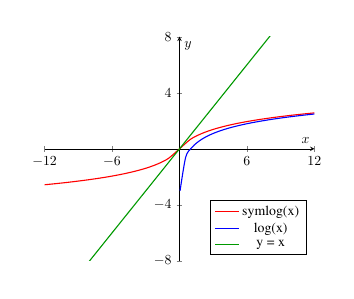
\begin{tikzpicture}[scale=0.5]
            \begin{axis}[
                axis lines = middle,
                xlabel = $x$,
                ylabel = $y$,
                xmin = -12, xmax = 12,
                ymin = -8, ymax = 8,
                xtick = {-12,-6,0,6,12},
                ytick = {-8,-4,0,4,8},
                legend pos = south east,
                smooth,
                domain = -12:12,
            ]
            \addplot[red, thick] {sign(x)*ln(abs(x) + 1)};
            \addplot[blue, thick, domain=0.05:12] {ln(x)};
            \addplot[green!60!black, thick] {x};
            \legend{\text{symlog}(x), \text{log}(x), y = x}
            \end{axis}
        \end{tikzpicture}
    \end{center}
\end{frame}

\begin{frame}
    \frametitle{Distributions - Uniform Mix}
    To prevent spikes, zero probabilities and inifite log probabilities in the KL loss, the categorical distributions (encoder, dynamics predictor, and actor distributions) are parametrized as mixtures \( 1\% \) of uniform and \( 99\% \) neural network output. 
    \[
        \mathbf{v}_{1:n} \leftarrow 0.99 \mathbf{v}_{1:n} + \frac{0.01}{n}
    \]
\end{frame}

\begin{frame}
    \frametitle{Distributions - Train Twoards Twohot Encoded Targets}
    In Dreamer V3, critics learn from symlog-transformed, twohot-encoded returns, improving the prediction accuracy for a wide range of return distributions. This enhancement aids in better value estimation and policy performance.
    \[ 
        \operatorname{twohot}(x)_i
        \doteq \begin{cases}
        |b_{k+1} - x| \,/\, |b_{k+1} - b_k| &\text{ if } i=k \\
        |b_{k\hphantom{+1}} - x| \,/\, |b_{k+1} - b_k| &\text{ if } i=k+1 \\
        0 &\text{ else} \\
        \end{cases} \qquad
        k \doteq \sum_{j=1}^{|B|} \operatorname{\delta}(b_j < x)
    \]

    For example, if \( b = [0, 2.5, 5, 7.5, 10] \), then \( \text{twohot}(5.5) = [0, 0, 0.8, 0.2, 0] \).
    
    Now the loss function for the critic is inroduced by:
    \[
        \mathcal{L}(\theta) \doteq
        - \text{twohot} (y) ^ {\intercal} \text{log} \text{ softmax} ( f(x, \theta) )
    \]
\end{frame}

\begin{frame}{RePo Model: the Insight}
    Authors of RePo (\cite{zhu2023reporesilientmodelbasedreinforcement}) purposes that a state \( s \) can consist of useful information \( s^{(1)} \) and distractors \( s^{(2)} \), where only \( s^{(1)} \) is related to the rewards. 

    Examples of \( s^{(2)} \) can be lighting conditions, moving backgrounds, these are espically critical in real-life situations.

    So the authors would want find a way to extract out the the informations that are not useful, and therefore increase the performance of the model.
\end{frame}

\begin{frame}{Mutal Infomation}
    The mutal inforamtion of two random variables \( X \) and \( Y \) is definied as:
    \[
        \mathbf{I}(X; Y) = \sum_{x \in \mathcal{X}, y \in \mathcal{Y}} p(x, y) \log\left(\frac{p(x, y)}{p(x)p(y)}\right)
    \]
    The range of mutal information is \( [0, \infty) \). Intuitively speaking, this can be regard as "how helpful is it given \( X \) to predict \( Y \)".
\end{frame}

\begin{frame}{Notations}
    Let us define the following notations:
    \begin{itemize}
        \item \( o_t \) denote the high-dimensional image observation at time \( t \),
        \item \( z_t \) be the latent representation obtained via an encoder,
        \item \( a_t \) be the action taken at time \( t \),
        \item \( r_t \) be the reward at time \( t \).
    \end{itemize}
\end{frame}


\begin{frame}{The Learning Problem}
    The authors of RePo suggests that to conduct:
    \[
        \max_{\phi} \mathbf{I}_{\phi}(z_{1:T}; r_{1:T} \mid a_{1:T}) ~~\text{s.t.}~~ \mathbf{I}_{\phi}(z_{1:T}; o_{1:T} \mid a_{1:T}) < \epsilon. 
    \]

    As maximizing \( \mathbf{I}(z_{1:T}; r_{1:T} \mid a_{1:T}) \) being a way to make the latent state information \( s_t \) useful by making it a information that is able to predict rewards, while \( \mathbf{I}(z_{1:T}; o_{1:T} \mid a_{1:T}) < \epsilon \) being a way to "filter out" some information related to the input image \( o_t \) that is not helpful for predicting rewards.
\end{frame}


\begin{frame}{The Learning Problem (Cont.)}
    It can be shown that:
    \begin{align*}
        \mathbf{I}_{\phi}(z_{1:T}; r_{1:T} \mid a_{1:T}) & \geq \mathbb{E}_{\phi} \left[ \sum_{t = 1}^T \text{log}\ q_\phi (r_t | z_t)  \right] \\
        \mathbf{I}_{\phi}(z_{1:T}; o_{1:T} \mid a_{1:T}) & \leq  \mathbb{E}_{\phi} \left[ \sum_{t = 0}^{T - 1} \KL[(\qp( \cdot |z_t,x_t, a_t)) || \pp( \cdot |z_t, a_t)] \right]
    \end{align*}

    And the original problem:
    \[
        \max_{\phi} \mathbf{I}_{\phi}(z_{1:T}; r_{1:T} \mid a_{1:T}) ~~\text{s.t.}~~ \mathbf{I}_{\phi}(z_{1:T}; o_{1:T} \mid a_{1:T}) < \epsilon. 
    \]
    can be transformed into:
    \[
        \max_{\phi} \mathbb{E}_{\phi} \left[ \sum_{t = 1}^T \text{log}\ q_\phi (r_t | z_t) \right] ~~\text{s.t.}~~ \mathbb{E}_{\phi} \left[ \sum_{t = 0}^{T - 1} \KL[(\qp( \cdot |z_t,x_t, a_t)) || \pp( \cdot |z_t, a_t)] \right] < \epsilon. 
    \]
\end{frame}

\begin{frame}{The Learning Problem (Cont.)}
    Then we can transform the problem into a Lagrangian optimization problem:
    \begin{align*}
        \max_{\phi} \min_{\beta} \Bigg\{ 
        & \mathbb{E}_{\phi} \left[ \sum_{t = 1}^T \text{log}\ q_\phi (r_t | z_t) \right] \\
        & + \beta \left( \mathbb{E}_{\phi} \left[ \sum_{t = 0}^{T - 1} \KL[(\pp( \cdot |z_t,x_t, a_t)) || \qp( \cdot |z_t, a_t)] \right] - \epsilon \right)
        \Bigg\}
    \end{align*}
    
    Then we can conduct dual gradient descent for this problem.
\end{frame}

\begin{frame}{Experiments}
    Environment: Atari100k Asterix. Trying to test:
    \begin{enumerate}
        \item The effect of adding noise on the input image while training Dreamer V3.
        \item If RePo outperforms Dreamer V3 in noisy environments.
    \end{enumerate}
\end{frame}

\begin{frame}{Experiments (Cont.)}
    Trained 3 Dreamer V3 models, for the input images, each of them received models that is added Gaussian noise of \( \sigma = 0, 10, 20 \). The scores are nearly identical when evaluating using clean images.

    \begin{center}
    \includegraphics[width=5 cm]{colors_dmr3.png}
    \end{center}

    \includegraphics[width=11cm]{eval_return_dmr3.png}
\end{frame}

\begin{frame}{Experiments (Cont.)}
    When inferencing these three models, with different kinds for input noise, these are the results.

    \begin{table}
        \centering
        \begin{tabular}{@{}l *{3}{c}@{}}
        \toprule
        \multirow{2}{*}[-0.5ex]{\makecell[l]{Model trained with}} & \multicolumn{3}{c}{Inference} \\
        \cmidrule(l){2-4}
        & $\sigma = 0$ & $\sigma = 10$ & $\sigma = 20$ \\
        \midrule
        $\sigma = 0$  & \(1091.67 \pm 50.94\) & \(996.67 \pm 141.36\) & \(1083.33 \pm 77.55\) \\
        $\sigma = 10$ & \(950.00 \pm 94.21\)  & \(875.00 \pm 151.38\) & \(916.66 \pm 107.44\) \\
        $\sigma = 20$ & \(916.66 \pm 92.91\)  & \(1008.33 \pm 97.87\) & \(958.33 \pm 83.42\) \\
        \bottomrule
        \end{tabular}
    \end{table}

    The experiments are inferenced with \( n = 12 \) and reported their \( 95\% \) confidence interval.
\end{frame}

\begin{frame}{Experiments (Cont.)}
    When trying to modify the code to the structure of RePo, the model isn't successful. Contrastive Loss should be around \( 10^{-2} \), but lots of models have the value around \( 10^8 \). There still need debugging.

    \includegraphics[width=9cm]{fail.png}
\end{frame}

\end{document}